
\chapter{Pipeline Assembly in Python}
\label{chap:pipeline}
This chapter links the preceding three chapters, illustrating assembling the different components into a functional pipeline.
An outline of the pipeline's operation and a discussion on certain design choices is presented.
The complete source code is available upon request.

% \section{Approach to Concurrency}
% As discussed in \ref{sec:concurrent_programming_in_python} using \gls{asyncio} is performant than using threads and offers more control over the execution and is therefore used to implement the pipeline.
% When the execution of external blocking code is required, it is wrapped in a \code{run_in_executor} call to run it in a thread pool.
% \gls{pygo} is callback-based,

% Several design patterns were tested during the development of the pipeline.
% In the final implementation

\section{Overall Structure}
The pipeline includes a synchronous setup phase, a concurrent running phase for executing multiple tasks, and a teardown phase for the graceful shutdown of all tasks.
Figure \ref{fig:object_overveiw} provides a high-level overview of the object in the pipeline and their interactions.

\gls{asyncio} is used to implement the concurrent running phase when possible, but certain tasks and callbacks are run in separate threads as this is required by some of the libraries used.


\subsection{Setup Phase}
\label{sec:discovery}

During the setup phase, the network manager ensures the Ethernet devices are configured as discussed in Section \ref{sec:network_configuration}.

Next, the camera manager is initialized to discover and configure the cameras.
Each Ethernet device has its own subnet where it attempts to find cameras.
If no cameras are detected, it searches the \gls{lla} subnet and configures any discovered camera to use an IP address within its subnet.

Once the cameras have been successfully discovered and configured, the Debayer Manager and GStreamer Manager, along with their respective pipelines, are initialized.

Finally, the video streams are initialized, and the running phase begins.

\subsection{Running Phase}
During the running phase, there are multiple concurrent tasks:

\begin{itemize}
    \item The \gls{ptp} Trigger continuously sends triggering signals to the cameras for simultaneous frame capture.
    \item Each Frame Grabber continuously grabs frames from the cameras and stores them in a queue.
    \item The Debayer Manager continuously retrieves frames from the queues, runs the debayer kernel and stores the output in a thread-safe queue.
    \item The Sink Pads, using callbacks, read data from the queues and pass it to the corresponding Pipeline when data is requested.
    \item The Src Pads, also using callbacks, pass available \gls{jpeg} data from the Pipeline to another thread-safe queue.
    \item An asynchronous \gls{ws} client forwards the \gls{jpeg} data to the PubSub Server discussed in Section \ref{sec:pubsub}.
    \item Another client listens to various camera setting topics and configures the cameras accordingly.
    \item The GStreamer Manager runs in a separate thread.
\end{itemize}



\subsection{Shutdown Phase}

When the pipeline receives a shutdown signal from the \srgui via the PubSub Server, it initiates the shutdown phase.
All tasks are instructed to stop, and the pipeline waits for their completion before terminating any remaining tasks.
Subsequently, the memory is freed, the streams are closed, and the \gls{ws} clients are disconnected.
The network settings and camera settings are not restored to minimize the startup time for subsequent runs.
Leaving the cameras with an IP within the corresponding Ethernet device's subnet ensures they are discovered much faster.


\begin{figure}[H]
    \centering
    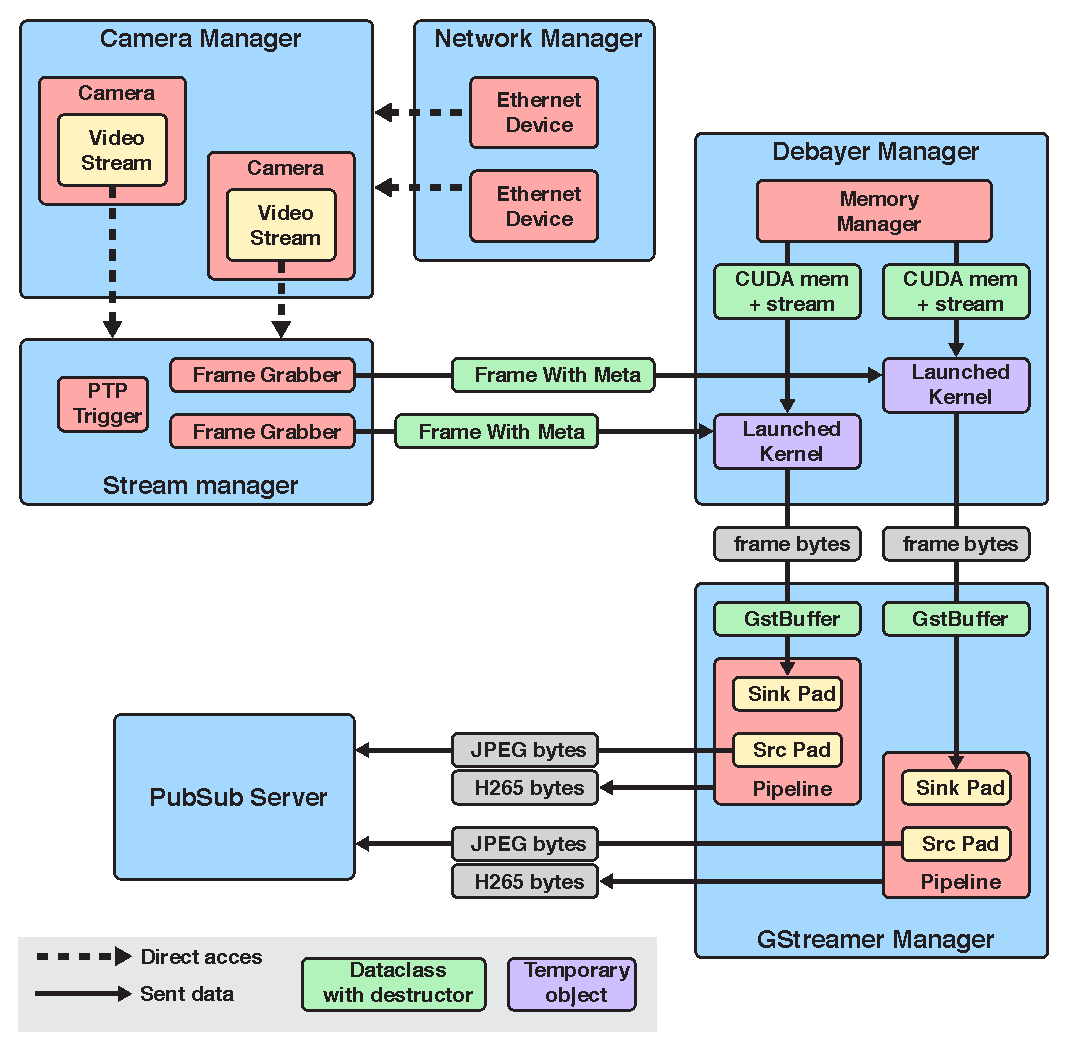
\includegraphics[width=\textwidth]{figures/object_overview.pdf}
    \caption{Class diagram showing the relationship between the classes in the pipeline and how thei interact.}
    \label{fig:object_overveiw}
\end{figure}

\section{Notes on Key Features}
Following are notes on some of the key features of the pipeline.

\subsection{Sharing Subcomponents}
To address synchronization challenges during object creation, configuration, and utilization, the pipeline employs a strategy where certain sets of elements are created, owned, and destroyed by one object but directly used by another.

The ethernet device objects are created, owned, and configured by the Network Manager and used by directly by the Camera Manager during the creation of each Camera object.
The Network Manager ensures that they never are configured to have overlapping subnets, as this causes issues during the discovery, creation, and operation of the cameras.

The Video Stream objects are created and configured by their corresponding camera object and used directly by the Video Stream Manager, which grabs frames and makes sure that the left and right frames are synchronized.

\subsection{Graceful Shutdown}
In real-time systems involving external hardware, it is essential to implement controlled shutdown procedures to avoid potential complications and issues in future runs.

On the \sr it is especially important to handle the camera and stream objects appropriately to avoid the cameras becoming inaccessible.
This is achieved by utilizing the \code{with} and \code{async with} syntax in Python, along with \code{try-finally} blocks, to ensure proper resource cleanup.

In case the cameras become inaccessible, a possible solution is to temporarily disable the Ethernet interface they are connected to for approximately two minutes.
This action appears to trigger an internal reset of the cameras, restoring their functionality.

\subsection{Custom Destructors}
Several custom message types have been developed with custom destructors to ensure proper cleanup.

The Frame With Meta object contains the data and relevant metadata for a single frame.
The underlying memory is managed internally by \gls{arena-api} and needs to be explicitly freed back to the underlying memory pool in order for new frames to be allocated.
This object has a custom \code{free} function used to free the underlying memory and \code{__del__} function that logs a warning if the memory has not been freed explicitly and frees it.

Allocating\gls{cuda} memory is a slow operation.
According to \gls{nsys}, allocating the necessary memory to perform the transformation presented in Chapter \ref{chap:debayer} takes more time than the transformation itself.
To avoid this overhead, a custom\gls{cuda} memory pool was implemented that r\gls{cuda} CUDA memory in order to avoid allocating and freeing memory and stream objects for each frame.
This pool is managed by the Memory Manager.
When the\gls{cuda} Memor\gls{cuda} CUDA Stream used by a kernel goes out of scope

Finally, \gls{gstreamer} uses its own garbage collection system and reference counting to manage memory.
Fortunately, the \gls{pygo} bindings for \gls{gstreamer} handles this automatically by having the python object participate in the reference counting, ensuring that the underlying \gls{gstreamer} object is not freed before the \py object is.


\subsection{Debayer Manager: Running CUDA Kernels in Python}
The main role of the debayer manager is to integrate the\gls{cuda} code with \py.
To achieve this, \gls{pybind11} was used.
\gls{pybind11} is a \gls{cpp} library that allows for the creation of \py bindings for \gls{cpp}, also \gls{cpp} funcions that launch \gls{cuda} kernels.

When working with \gls{cuda}, the easiest way to get data from \py was to pass pointers to the underlying data of the \gls{numpy} and \gls{cupy} arrays.
These pointers are available as inegers through the \code{__array_interface__} and \code{__cuda_array_interface__} respectively \cite{numpyArrayInterfaceProtocol} \cite{cupyInteroperabilityCuPy12}.
This allows for zero-copy data transfer between \gls{cuda} and \py, but requires manual interpretation of the data structure on the \gls{cpp} side and should be done with caution as it is easy to get segmentation faults.

Passing data as \gls{eigen} arrays without copying the data was also achieved, and the \gls{eigen} arrays could be used directly in \gls{cuda} \cite{wenzelEigenPybind11Documentation2017} \cite{eigenEigenUsingEigen}.
While this was a more memory-safe way to transfer data required a lot more boilerplate on the \gls{cpp} side and was slower than passing pointers to the underlying data.


It is worth mentioning that it is also possible to write \gls{cuda} kernels in \py directly through \gls{cupy} as well as other \gls{gpu} accelerated libraries such as \gls{numba} and \gls{pytorch}
Based on prioer experience, however, these are impossible to debug and should be avoided for anything but the simplest of tasks.